\documentclass{amsbook}
\usepackage{graphicx}
\usepackage{./HBSuerDemir}

\begin{document}

\hPage{b1p2/302} 
\pagenumbering{gobble}

\subsection*{\underline{Example 1}} Transform the cartesian equation to polar one:
\begin{equation*}
	a) ax + by + c = 0 (line) b) x^2 + y^2 - 2ax = 0 (circle)
\end{equation*} 

\subsection*{\underline{Solution}} 
Setting $x = r cos\theta$, $y = r sin\theta$, we have \\

\begin{itemize}
    \item [a)] $ar\ cos\theta + br\ \sin\theta + c = 0 \Rightarrow r = \frac{c}{a \cos\theta + b \sin\theta}$
    \item [b)] $r^2 - 2ar cos\theta \Rightarrow r (r - 2a cos\theta) = 0 \Rightarrow r = 0$ (pole) or $r = 2a cos\theta$. But $r = 0$ is contained in the second for $\theta = \pi/2$. Hence transformed equation is $r = 2a cos\theta$.
\end{itemize}

\subsection*{\underline{Example 2}} Transform the polar equation to cartesian:

\begin{itemize}
    \item[a)]  $r = a (1 + cos\theta)$ (cardioid)
    b) $r^2 = a^2 \cos{2\theta}$ (lemniscate)
\end{itemize}

\subsection*{\underline{Solution}} 

\begin{itemize}
    \item[a)] We express first $cos\theta$ in terms of x and r and then replace $r^2$ by $x^2$ + $y^2$:
    \begin{align*}
    r = a (1 + cos\theta) &\Rightarrow r = a (1 + \frac{x}{r}) \Rightarrow r^2 = a (r + x) \\
    x^2 + y^2 = ar + ax &\Rightarrow (x^2 + y^2 - ax)^2 \Rightarrow a^2 (x^2 + y^2).
    \end{align*}

    \item[b)]
    \begin{align*}
    x^2 &= a^2 cos{2\theta} \Rightarrow x^2 + y^2 = a^2(cos{2}{\theta} - sin{2}{\theta}) \\
    x^2 &+ y^2 = a^2(\frac{x^2}{r^2} - \frac{y^2}{r^2}) \Rightarrow (x^2 + y^2)^2 = a^2 (x^2 - y^2)
    \end{align*}
    
\end{itemize}

\subsection*{\underline{Example 3}} Write two representations of points A, B, C, D, E, F in the given figure, where OAB, OCD are equilateral triangles, and OEFA is, a square ($\abs{OA} = 2$, $\abs{OD} = 3$)

\subsection*{\underline{Solution}} Since $\abs{OA} = \abs{OB} = 2$, $\abs{OC} = \abs{OD} = 3$, we have form Figure,

\noindent $A (0 , 2) = A (\pi, -2)$ \\
$B (\frac{\pi}{3} , 2) = B (\frac{\pi}{3} + \pi, -2)$ \\
$C (2\frac{\pi}{3} , 3) = C (-\frac{\pi}{3} , -3)$ \\
$D (\pi , 3) = D (0 , -3)$ \\

\begin{figure}[h]
    \begin{minipage}{0.5\linewidth}
        \centering
        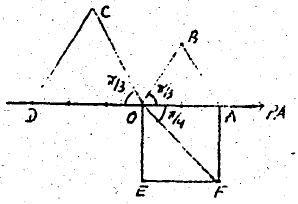
\includegraphics[width = 0.80\textwidth]{images/b1p2-302-fig01}
    \end{minipage}
\end{figure}

\end{document}
